
\begin{figure}
\begin{minipage}[height=.3\textheight]{.32\textwidth}
\centering \small{\texttt{(a)}}
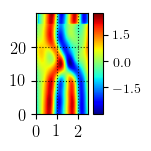
\includegraphics[width=1.0\textwidth,height=.25\textheight]{MNG_HOD_init}
\end{minipage}
\begin{minipage}[height=.3\textheight]{.32\textwidth}
\centering \small{\texttt{(b)}}
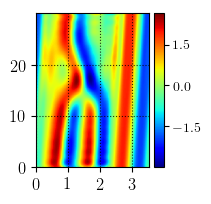
\includegraphics[width=1.0\textwidth,height=.29\textheight]{MNG_HOD_STREAK_init}
\end{minipage}
\begin{minipage}[height=.3\textheight]{.32\textwidth}
\centering \small{\texttt{(c)}}
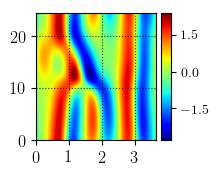
\includegraphics[width=1.0\textwidth,height=.17\textheight]{MNG_HOD_STREAK_final}
\end{minipage}
\caption{ \label{fig:MNGhodstreak}
(a) Initial condition from \reffig{fig:MNG_HOD_tile} that converges to
a solution that is believed to be a numerical continuation of (b) from \reffig{fig:MNGsymb11}. (b) An initial condition
resulting from concatenating a streak-pair with (a), that
numerically converges to (c).
}
\end{figure}

\begin{figure}
\begin{minipage}[height=.3\textheight]{.32\textwidth}
\centering \small{\texttt{(a)}}
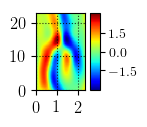
\includegraphics[width=1.0\textwidth,height=.25\textheight]{MNG_HD_init}
\end{minipage}
\begin{minipage}[height=.3\textheight]{.32\textwidth}
\centering \small{\texttt{(b)}}
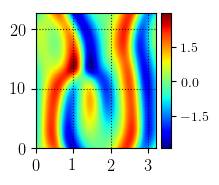
\includegraphics[width=1.0\textwidth,height=.29\textheight]{MNG_HD_STREAK_final}
\end{minipage}
\begin{minipage}[height=.3\textheight]{.32\textwidth}
\centering \small{\texttt{(c)}}
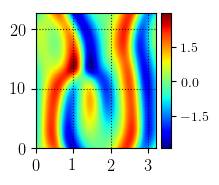
\includegraphics[width=1.0\textwidth,height=.17\textheight]{MNG_HD_STREAK_final}
\end{minipage}
\caption{ \label{fig:MNGhdstreak}
(a) Initial condition that has not been shown to numerically converge. (b) An initial condition
resulting from concatenating a streak-pair with (a), that
numerically converges to (c).
}
\end{figure}



\begin{figure}
\begin{minipage}[height=.4\textheight]{.5\textwidth}
\centering \small{\texttt{(a)}}\\
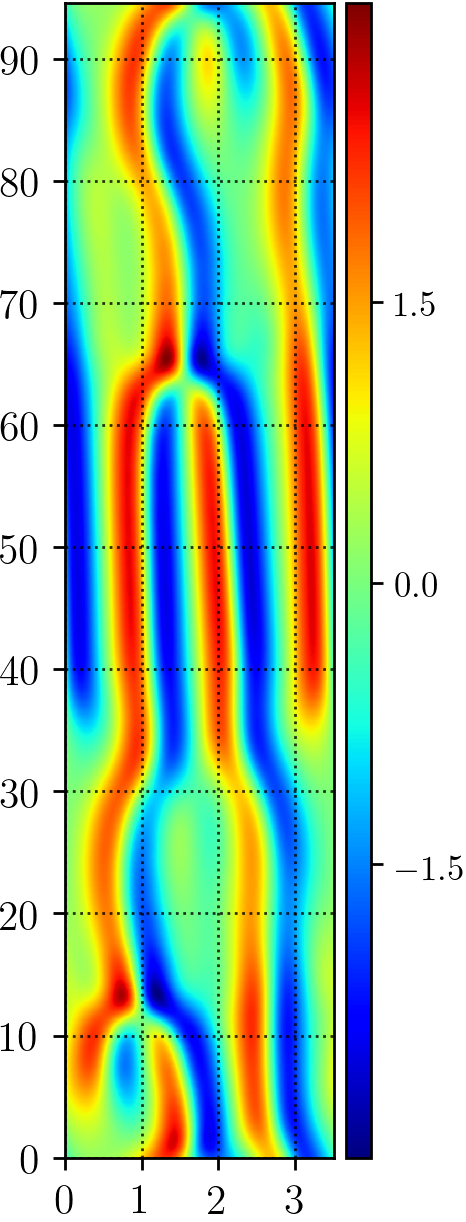
\includegraphics[width=.5\textwidth,height=.5\textheight]{MNG_halfdefect_defect_initial}
\end{minipage}
\begin{minipage}[height=.4\textheight]{.5\textwidth}
\centering \small{\texttt{(b)}}\\
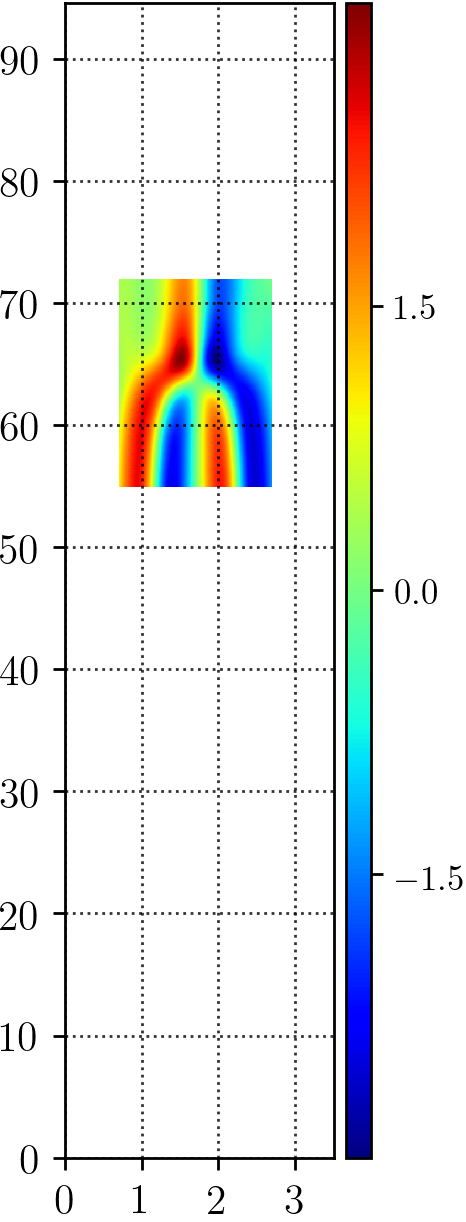
\includegraphics[width=.5\textwidth,height=.5\textheight]{MNG_defect_guess}
\end{minipage}
\begin{minipage}[height=.1\textheight]{\textwidth}
\centering \small{\texttt{(c)}}\\
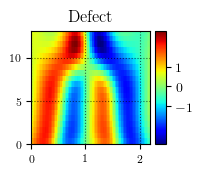
\includegraphics[width=.14\textwidth,height=.1\textheight]{MNG_defect}
\end{minipage}
\caption{ \label{fig:defect}
(a)
$[\speriod{a},\period{a}]=[3.50\cdots,94.59\cdots]$ fundamental domain
of an already computed \twot\ with spatial translation symmetry.
(b)
The clipped-out $[\speriod{b},\period{b}]=[2,17]$ subdomain used the
initial guess for the fundamental domain of a shift-reflect symmetric tile.
(c)
The converged $[\speriod{c},2\period{c}]=[2.07\cdots,18.46\cdots]$ \twot\
with spatial translation symmetry.
}
\end{figure}

\begin{figure}
\begin{minipage}[height=.4\textheight]{.5\textwidth}
\centering \small{\texttt{(a)}}\\
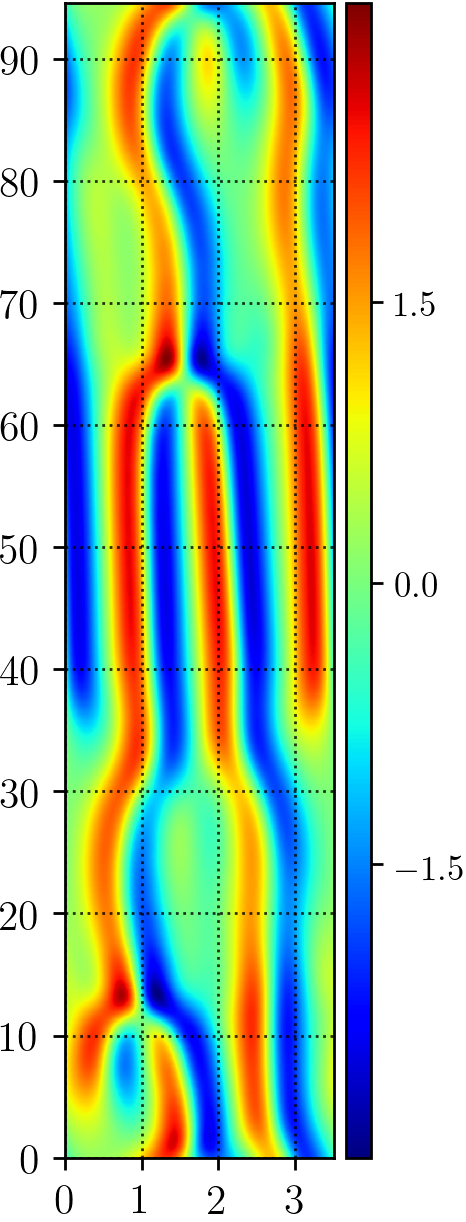
\includegraphics[width=.5\textwidth,height=.5\textheight]{MNG_halfdefect_defect_initial}
\end{minipage}
\begin{minipage}[height=.4\textheight]{.5\textwidth}
\centering \small{\texttt{(b)}}\\
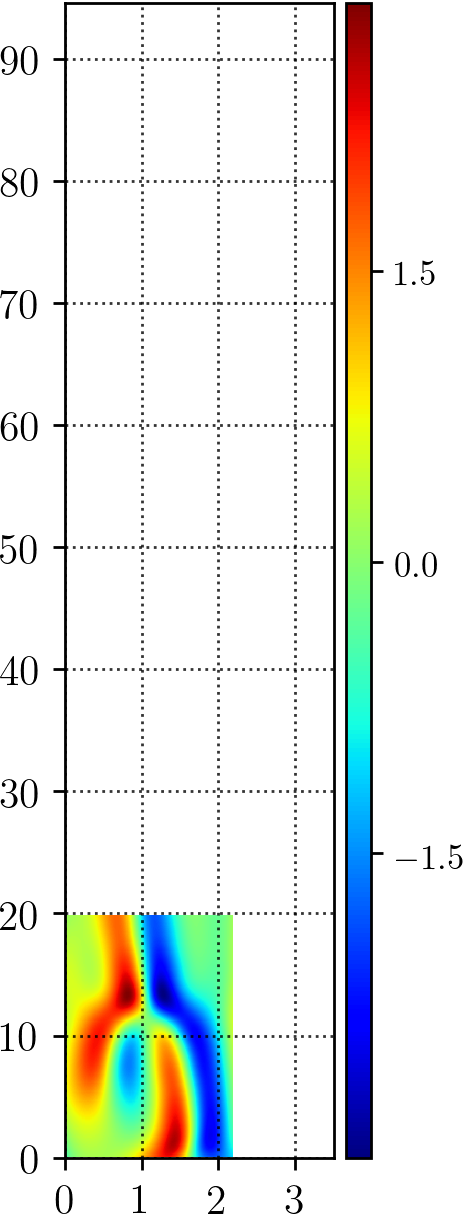
\includegraphics[width=.5\textwidth,height=.5\textheight]{MNG_halfdefect_guess}
\end{minipage}
\begin{minipage}[height=.1\textheight]{\textwidth}
\centering \small{\texttt{(c)}}\\
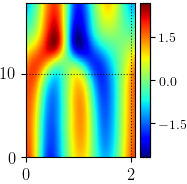
\includegraphics[width=.14\textwidth,height=.12\textheight]{MNG_halfdefect}
\end{minipage}
\caption{ \label{fig:halfdefect}
(a)
$[\speriod{a},\period{a}]=[3.50\cdots,94.59\cdots]$ fundamental domain
of an already computed \twot\ with spatial translation symmetry.
(b)
The clipped-out $[\speriod{b},\period{b}]=[2.2,20]$ subdomain used the
initial guess for the fundamental domain of a shift-reflect symmetric tile.
(c)
The converged $[\speriod{c},2\period{c}]=[2.07\cdots,15.46\cdots]$ \twot\
with spatial translation symmetry.
}
\end{figure}

\begin{figure}
\begin{minipage}[height=.4\textheight]{.5\textwidth}
\centering \small{\texttt{(a)}}\\
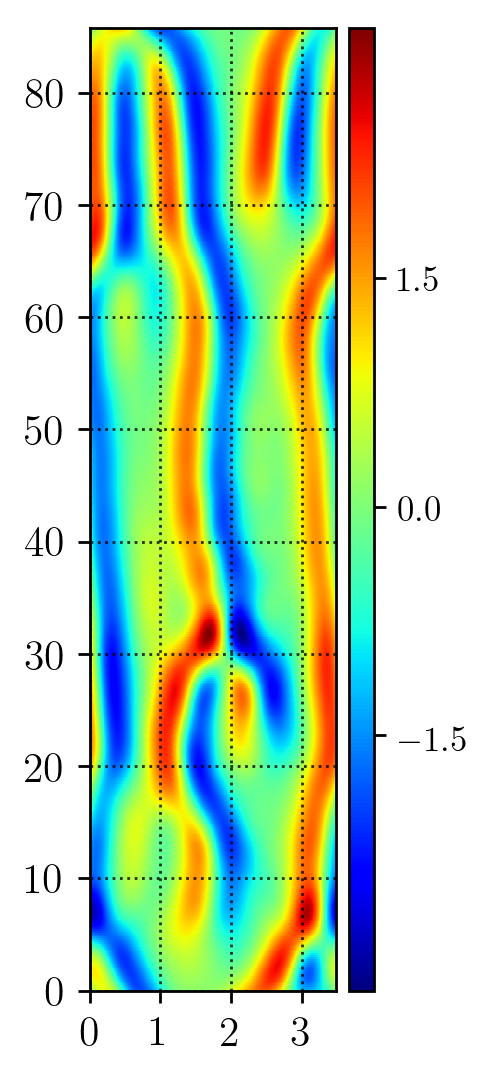
\includegraphics[width=.5\textwidth,height=.5\textheight]{MNG_halfdefect2_initial}
\end{minipage}
\begin{minipage}[height=.4\textheight]{.5\textwidth}
\centering \small{\texttt{(b)}}\\
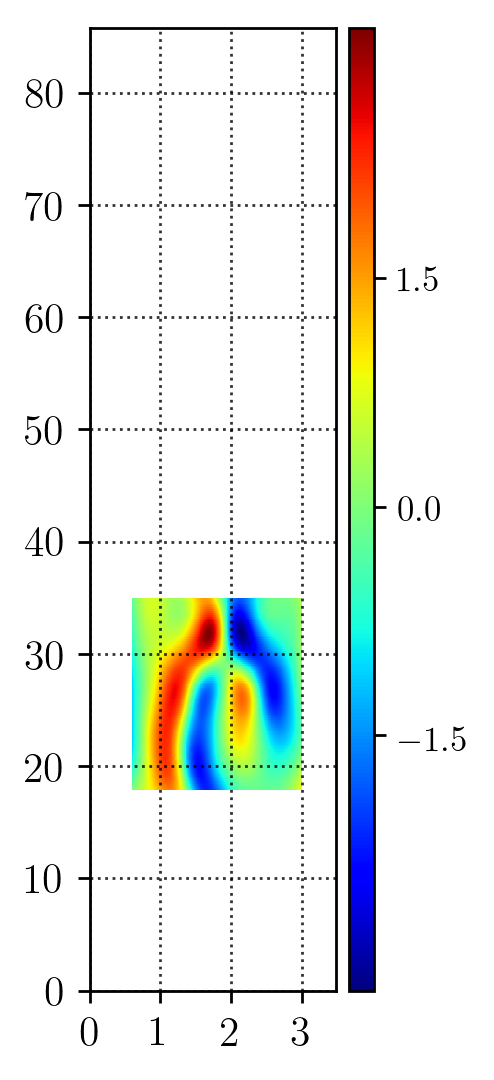
\includegraphics[width=.5\textwidth,height=.5\textheight]{MNG_halfdefect2_guess}
\end{minipage}
\begin{minipage}[height=.1\textheight]{\textwidth}
\centering \small{\texttt{(c)}}\\
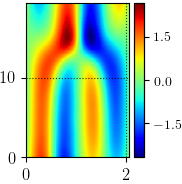
\includegraphics[width=.14\textwidth,height=.1\textheight]{MNG_halfdefect2}
\end{minipage}
\caption{ \label{fig:halfdefect2}
(a)
$[\speriod{a},\period{a}]=[3.50\cdots,85.73\cdots]$ fundamental domain
of an already computed \twot\ with \spt\ shift-reflection symmetry.
(b)
The clipped-out $[\speriod{b},\period{b}]=[2.6,17]$ subdomain used the
initial guess for the fundamental domain of a shift-reflect symmetric tile.
(c)
The converged $[\speriod{c},\period{c}]=[2.06\cdots,19.92\cdots]$ \twot\
with spatial translation symmetry.
}
\end{figure}

\begin{figure}
\begin{minipage}[height=.1\textheight]{.5\textwidth}
\centering \small{\texttt{(a)}}\\
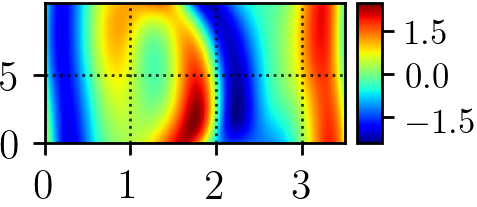
\includegraphics[width=.5\textwidth,height=.1\textheight]{MNG_hook_initial}
\end{minipage}
\begin{minipage}[height=.1\textheight]{.5\textwidth}
\centering \small{\texttt{(b)}}\\
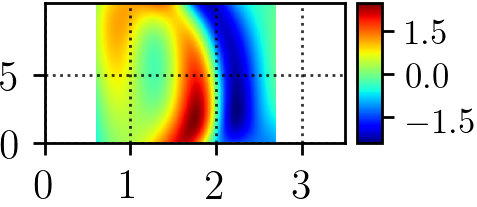
\includegraphics[width=.5\textwidth,height=.1\textheight]{MNG_hook_guess}
\end{minipage}
\begin{minipage}[height=.1\textheight]{\textwidth}
\centering \small{\texttt{(c)}}\\
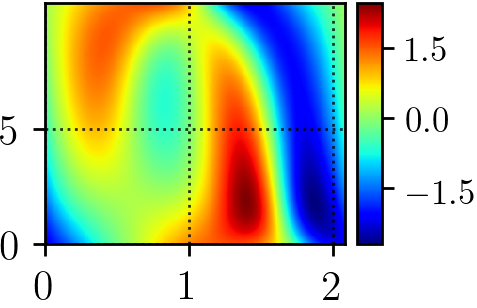
\includegraphics[width=.16\textwidth,height=.1\textheight]{MNG_hook}
\end{minipage}
\caption{ \label{fig:hook}
(a)
$[\speriod{a},\period{a}]=[3.50\cdots,10.25\cdots]$ fundamental domain
of an already computed \twot\ with \spt\ shift-reflection symmetry.
(b)
The clipped-out $[\speriod{b},\period{b}]=[2.1,10.5]$ subdomain used the
initial guess for the fundamental domain of a shift-reflect symmetric tile.
(c)
The converged $[\speriod{c},\period{c}]=[2.08\cdots,9.22\cdots]$  \twot\
with spatial translation symmetry.
}
\end{figure}

\begin{figure}
\begin{minipage}[height=.3\textheight]{.5\textwidth}
\centering \small{\texttt{(a)}}\\
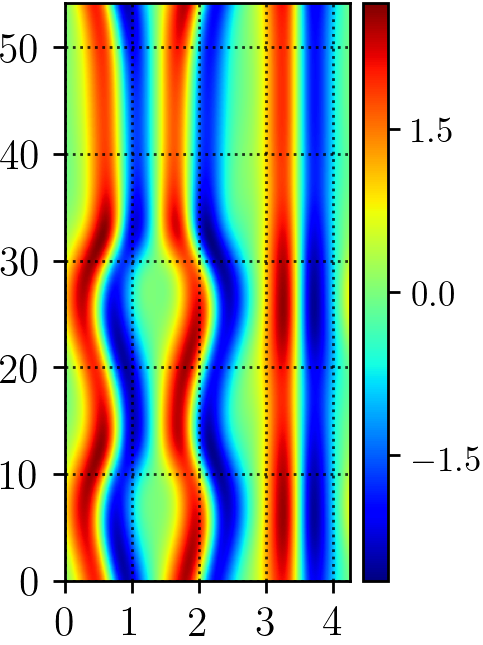
\includegraphics[width=.6\textwidth,height=.4\textheight]{MNG_gap_initial}
\end{minipage}
\begin{minipage}[height=.3\textheight]{.5\textwidth}
\centering \small{\texttt{(b)}}\\
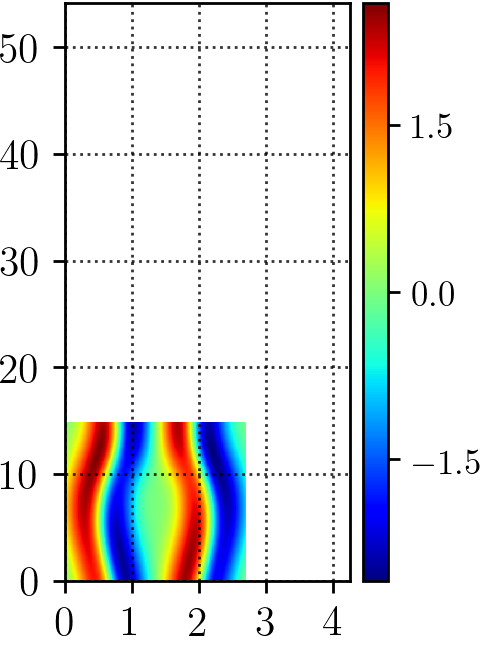
\includegraphics[width=.6\textwidth,height=.4\textheight]{MNG_gap_guess}
\end{minipage}
\begin{minipage}[height=.1\textheight]{\textwidth}
\centering \small{\texttt{(c)}}\\
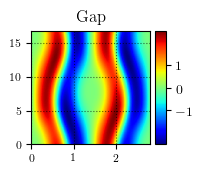
\includegraphics[width=.12\textwidth,height=.13\textheight]{MNG_gap}
\end{minipage}
\caption{ \label{fig:gap}
(a)
$[\speriod{a},\period{a}]=[4.25\cdots,54.13\cdots]$ fundamental domain
of an already computed \twot\ with \spt\ shift-reflection symmetry.
(b)
The clipped-out $[\speriod{b},\period{b}]=[2.7,15]$ subdomain used the
initial guess for the fundamental domain of a shift-reflect symmetric tile.
(c)
The converged $[\speriod{c},\period{c}]=[2.90\cdots,17.95\cdots]$ full
reflection symmetric \twot.
}
\end{figure}

\begin{figure}
\begin{minipage}[height=.2\textheight]{.5\textwidth}
\centering \small{\texttt{(a)}}\\
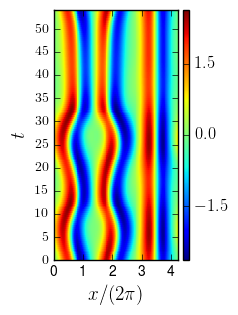
\includegraphics[width=.8\textwidth,height=.5\textheight]{MNGgapzero}
\end{minipage}
\begin{minipage}[height=.2\textheight]{.5\textwidth}
\centering \small{\texttt{(b)}}\\
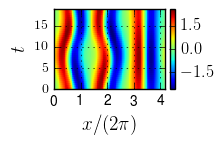
\includegraphics[width=.8\textwidth,height=.18\textheight]{MNGgapone}
\end{minipage}
\begin{minipage}[height=.2\textheight]{.5\textwidth}
\centering \small{\texttt{(c)}}\\
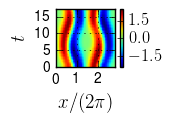
\includegraphics[width=.6\textwidth,height=.18\textheight]{MNGgaptwo}
\end{minipage}
\begin{minipage}[height=.2\textheight]{.48\textwidth}
\centering \small{\texttt{(d)}}\\
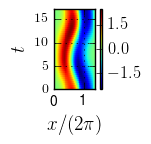
\includegraphics[width=.5\textwidth,height=.18\textheight]{MNGgapthree}
\end{minipage}
\caption{ \label{fig:KStileextraction}
Sequential subdomain extraction to find tiles.
(a) A {\po} from the collection of new solutions
$[\speriod{a},\period{a}]=[4.25\cdots,54.12\cdots]$.
By taking progressively smaller subdomains (b)-(d) and numerically
converging them to \twots\ at each step, we are able to
find the smallest subdomain of (a) which can be converges
to a \twot, namely (d).
(b)$[\speriod{b},\period{b}]=[4.16\cdots,18.93\cdots]$
(c)$[\speriod{c},\period{c}]=[2.79\cdots,17.14\cdots]$
(d)$[\speriod{d},\period{d}]=[1.39\cdots,17.14\cdots]$
}
\end{figure}